\begin{abstract}
%%%  Matt
The DUNE physics program is highly heterogeneous with important goals in beam physics, SuperNova burst neutrino detection and the related topics of nucleon decay and non-beam neutrinos.
Each of these topics requires a different data acquisition strategy for identifying and storing the relevant part of the 10 Tb/s stream of data coming from each 17 kT LArTPC module. 
Consequently, the DAQ system for the DUNE Far Detector LArTPC must be flexible and highly performant to meet all of these requirements.
This note describes a modest evolution of the system already demonstrated at the ProtoDUNE-SP detector that meets all of these requirements. 
It is based on the RCE/ATCA system developed at SLAC. 
Because the major components of this system have already been demonstrated, a relatively small additional development effort is needed to extend its performance to that needed for the DUNE-FD. 
Adopting this system minimizes the technical risk and design costs and thus represents a very attractive technical solution.

\end{abstract}

\section{Introduction}
\label{sec:introduction}
(some intro stuff, some high level )

The DAQ design (focusing on the TPC) must meet the following requirements:
\begin{itemize}
\item{trigger on activity in the TPC and store $\sim$5ms of unsuppressed TPC data per trigger}
\item{other stuff..this must be written down in TP}
\item{constantly buffer, unsuppressed, at least 10s of all TPC data in anticipation of a prompt supernova trigger}
\item{maintain an DAQ-related uptime of $>$99\%}
\end{itemize}
Please note that these requirements are in the process being refined.  

The DUNE DAQ high-level design include 3 parts:  the front-end readout, the trigger system, and the back-end readout.  While the entire DAQ system is responsible for reading out both the TPC and the Photon Detector, this note focuses on the TPC readout.  The RCE-system described here would cover the front-end part of the TPC DAQ design (though some of the extensions described in the last section include functionality that could be considered part of the trigger and back-end systems).   The front-end DAQ system is responsible for:

\begin{itemize}
\item  reading out the TPC front-end and dealing with errors in the readout
\item  performing trigger primitive finding and forwarding to trigger system
\item (if required/desired) performing lossless compression of the data
\item buffering the data for an extended period and sending a certain time slice to the backend DAQ upon receipt of a trigger message (this includes buffering while waiting for a SN trigger)
\end{itemize}

In this note we will describe a DAQ design based around the RCE/ATCA platform reading out the TPC front-end.  We begin by detailing the RCE, COB, and ATCA hardware in Section \ref{sec:RCEPlatformOverview}, followed by describing the existing firmware (Section \ref{sec:firmware}) and software (Section \ref{sec:software}).  

This note uses many acronyms; please see Table \ref{tab:acronym} for a list of commonly used ones.  

\begin{table}[htp]
\begin{center}
\begin{tabular}{|c|c|}
\hline
Acronym  &  Full Name \\
\hline
\hline
APA  & Anode Plane Assembly\\
\hline
FEMB  & Front End Mother Board\\
\hline
WIB  &  Warm Interface Board  \\
\hline
ATCA  &  Advanced TeleCommunications Architecture\\
\hline
RTM  & Rear Transmission Module  \\
\hline
COB  &  Cluster On Board  \\
\hline
DTM  &  Data Timing/Trigger Module  \\
\hline
DPM  &  Data Processing Module  \\
\hline
RCE  &  Reconfigurable Cluster Element\\
\hline
%SOC  & System-On-Chip   \\
%\hline
\end{tabular}
\end{center}
\caption{List of acronyms used frequently in this note.  }
\label{tab:acronym}
\end{table}%


\subsection{Overview of the RCE/ATCA Design }



The RCE/ATCA system is at it's core a number of interconnected SOCs residing on  ATCA blades in an industry standard ATCA shelf.   The SOCs are on daughter boards (DPMs),  four to an ATCA blade, and include at least 8GB of attached memory.  The ATCA blade, called a Cluster-On-Board (COB), is a high-bandwidth device utilizing the MGTs on the SOCs for high-speed IO and a 10-Gbps ethernet switch connecting each RCE to each other and having 4 10-Gbps ports out of the COB\footnote{A version of the COB with a 40 Gbps switch is currently under design.} .  


The design shown in Figure \ref{fig:base} is an evolution of those used for the 35-ton and then protoDUNE prototype DAQs.  The additional features for the DUNE DAQ include:
\begin{itemize}
    \item an upgraded COB with 8x10Gbps or 8x40Gbps ethernet ports (note:  this was developed and built for the LSST experiment) 
    \item an upgraded SOC on the RCE with somewhat more FPGA resources, improved memory bandwidth and DDR4 compatibility, and an improved CPU
    \item at least 8GB DDR4  memory/RCE (up from 1GB DDR3) and a PCIe connected NVMe SSD for triggered supernova buffering\cite{SNBuff}
    \item a trigger-primitive data path with firmware performing filtering and hit-finding on incoming wave-forms and streaming to a trigger decision cluster
    \item a supernova path which, upon receipt of a supernova trigger, sends data to the onboard SSD for a fixed number of seconds and then trickles the data out to a backend system
\end{itemize}
The other features of Figure \ref{fig:base}, e.g. data receiving, compression, buffering etc., have all been implemented in the protoDUNE DAQ and would require only minor changes to implement for DUNE.  

In the base RCE/ATCA design described here, the only data that flows out of the ATCA shelf are the trigger primitives, to be processed by the trigger system PCs,, the triggered data itself, to be built into events and stored (or processed further in a software filter).  A summary of the COB input and output numbers are shown in Table \ref{tab:hsIO}.  

\begin{figure}[tb]
\centering
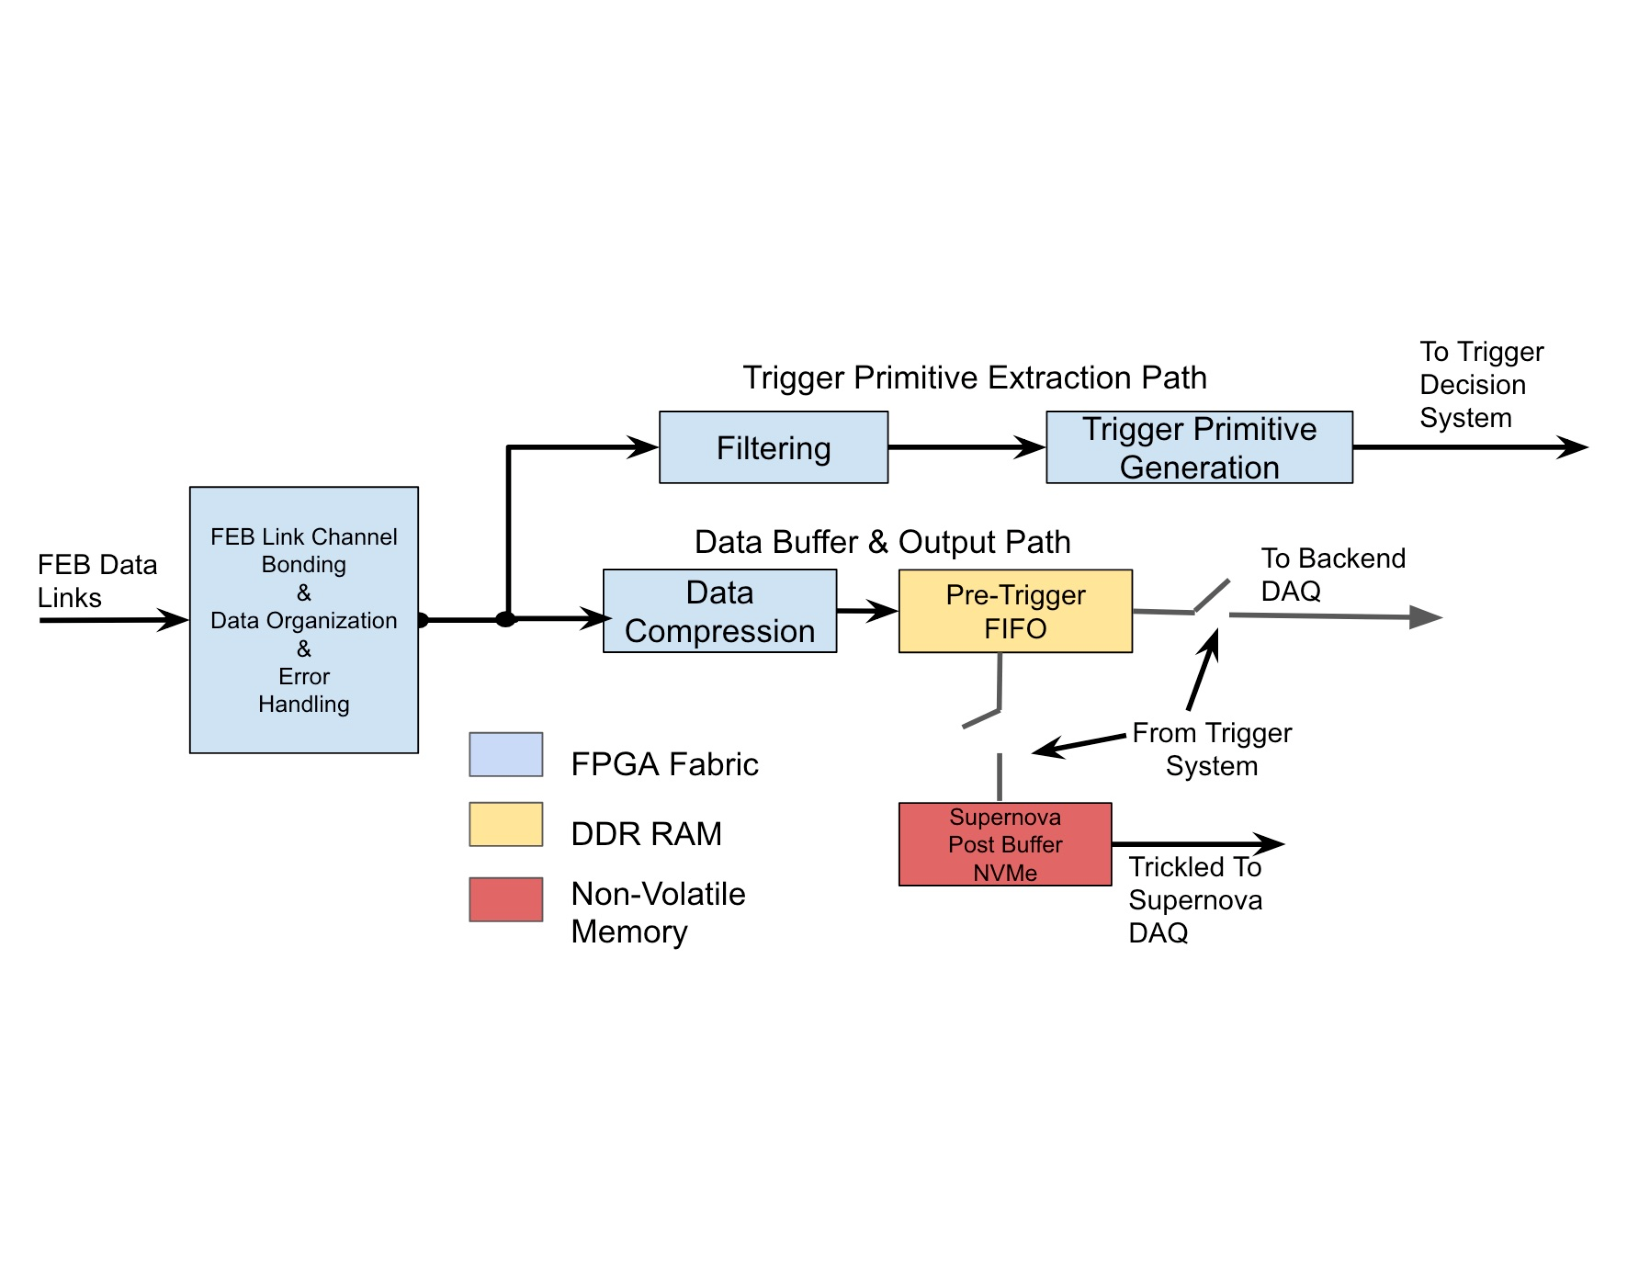
\includegraphics[width=1.0\textwidth]{images/base_rce_dune_dataflow.pdf}
\caption{\label{fig:base}Block diagram of of data flow in the RCE from the WIBs and to the trigger and backend DAQ systems. }
\end{figure}



\begin{table}[htp]
\begin{center}
\begin{tabular}{|c|c|c|}
\hline
     & Number/COB           &     Bandwidth/Link \\
     \hline
\multicolumn{3}{|l|}{\bf{Maximum for COB}} \\
\hline
High Speed I/O via RTM & 96 & 10 Gbps \\
Ethernet via Front Board & 8  & 10 Gbps \\
\hline
\multicolumn{3}{|l|}{\bf{Proposed for DUNE SP}} \\
\hline
TPC Data from WIBs via RTM & 20 & $\sim$5 Gbps\\
Trigger Primitives out via Ethernet  &  1*  &  $\sim$1 Gbps**** \\
Triggered Data out via Ethernet  &  1* &  $\sim$0.5 Gbps**** \\
Triggered SN Data out via Ethernet  & 1   &  $\sim$0.0 -10 Gbps\\
\hline
\end{tabular}
\end{center}
\caption{Summary of data connections and estimated bandwidths in and out of COB. This assumes 1 COB/APA.  Note that triggered primitives and triggered data would likely go over the same physical link (possibly the SN Data out as well).  }
\label{tab:hsIO}
\end{table}%

\begin{table}[htp]
\begin{center}
\begin{tabular}{|c|c|c|}
\hline
     & Number           &     Units \\
     \hline
\multicolumn{3}{|l|}{\bf{Front-End Electronics}} \\
\hline
TPC Channels & 128 & /FEMB \\
FEMBs  & 20  & /APA \\
FEMBs  & 4  & /WIB  \\
WIBs  & 5  & /APA\\
WIB Output Links* & 4 & /WIB\\
WIB Data Bandwidth* & $\sim$3.5 Gbps & /Link\\
\hline
\multicolumn{3}{|l|}{\bf{WIB-RCE Interface and RCEs}} \\
\hline
WIB Links into RTM & 20 & /COB\\
RCEs    & 4  &  /COB\\
WIB Links into RCE & 5 & /RCE\\
Data Bandwidth into RCE & 17.5 Gbps & /RCE\\
DDR4 Memory    & 8 GB & /RCE\\
Compression Factor (assumed)  & 3  &  \\
Buffer Depth (no compression)   &  $\sim$3.8  &  s  \\
Buffer Depth (with compression)   &  $\sim$11  &  s  \\
SSD Write Speed (measured)  & 1.6 & GBps \\ 
SN Dump Time (no compression)  &  $\sim$ 15  & s\\
SN Dump Time (with compression)  &  $\infty$  & s\\
\hline
\end{tabular}
\end{center}
\caption{ Numbers pertaining to the RCE/ATCA part of the DAQ assuming 1 COB/APA using the Oxford/SLAC Ultrascale+ RCE.  Note FEMB=Front-End Mother Board; WIB=Warm-Interface Board.  The WIBs output link configuring has not been settled yet, though we prefer to use 4-5Gbps links (each link = 1 FEMB).  The TPC data + headers on these links is listed in the table and is ~3.5 Gbps. }
\label{tab:apaNums}
\end{table}%



%The advantages of the RCE/ATCA design over a PC/software only design include: 
%\begin{itemize}
%\item some amazing points
%\end{itemize}




% %%%  Mark
% Being ready to detect and accurately measure burst neutrinos from a Galactic supernova is one of the major scientific goals of DUNE. On the order of 1,000-10,000 neutrino interactions are expected, given the range of distances in the galaxy and variations among  progenitor stars.  With such large statistics, it is possible to investigate not only the total emission, but also second-by-second evolution of the energy spectra. It is this time evolution of the signal that contains a potential gold mine of physics information. After all, since neutrinos come directly from the surface of the collapsed core, they carry real-time information about the unfolding explosion. One expects, for example, to be able to observe how the shock breaks through the neutrinosphere, where it stalls, how much matter is accreted during this stalled phase, when the shock is finally pushed out, and how it travels through the outer layers of the star. Formation of a black hole would also leave an imprint in neutrinos, as would phase transitions in the dense matter of the protoneutron star, late-time fall-back of material, novel energy-loss effects due to new physics, etc. 

% To reliably identify and interpret signatures of many of these phenomena, accurate neutrino energy reconstruction is required. This, however, is not a simple task. Although the bulk of the neutrino flux is expected to come in the energy range of 10-20 MeV, the strong energy dependence of weak interaction cross sections makes the neutrinos on the high-energy tail the main contributors to the signal.  The average energy of interacting neutrinos can be in the range of 25-35 MeV and even events with energies as high as 50-60 MeV are predicted in several oscillation scenarios. Nuclear physics models of $\nu-Ar$ scattering at 25-50 MeV predict highly nontrivial final states, with the energy distributed between final-state electrons, de-excitation gammas and knock-out neutrons. While electrons may be relatively easy to trigger on, some or all of de-excitation gammas could end up zero-suppressed, if the event identification were to be handled on line. Moreover, neutrons are expected to random-walk some distance away, perhaps as far as 2 m, and finally capture out of time with the original interaction. 

% Since accurate reconstruction of neutrino energies requires identification of all of the final state particles, it is vastly preferable to save all the information from the detector during the burst time window, rather than depend on the algorithm to make decisions online. With full data safely stored, the collaboration (and humankind) will have years and decades to comb through the data.

% The next logical question has to do with the duration of the time window that should be saved. Given that the SN 1987A neutrino signal lasted 12 seconds, we clearly should not even consider anything shorter than that. In fact, it makes good sense to save data beyond 12 seconds. This way we will have a chance to look for phenomena such as late-time fall-back, phase transitions in the core of the cooling protoneutron star,  or even late-time black hole formation. Thus, one would like, in principle, to save on the order of 60-100 seconds of the full detector readout, unless the costs of doing so somehow becomes prohibitive. In fact, it does not; below, we show how this can be accomplished, with a technically robust and cost-effective design.

% \section{Double Buffer Concept}
% %%%  Matt/Mark

% \begin{figure}[h]
% \centering
% 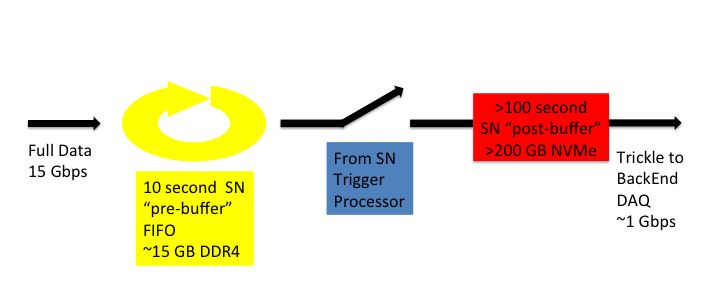
\includegraphics[width=0.9\textwidth]{images/Slide1.png}
% \caption{\label{fig:concept}Concept for "double buffering" SN data. This layout would be reproduced in each of the 600 RCEs (or equivalent). (NOTE: Need to adjust DDR size)}
% \end{figure}

% The previous section has made it clear that, in the event of a galactic SN it is desirable to save the entire, non-zero-suppressed data stream to long term storage for a period of ~100 seconds. 
% The full data stream will be about 9 Tb/s of ADC data for one single-phase 10kT module. 
% Various overheads raise this rate to between 12 and 15 Tb/s.
% The DUNE Technical Proposal assumes 12 Tb/s of TPC data, so will use that rate for the rest of this note.
% The primary data stream of the DUNE DAQ system will not be capable of writing this amount of data in "real time". 
% The back-end network and storage bandwidths would both be much larger than needed for any other type of physics, and thus would be prohibitively expensive.

% However, as discussed in Section \ref{sec:sntrigger},
% we expect to be able to trigger efficiently on galactic SN bursts with a latency of approximately one second. 
% We can imagine buffering the full datastream for 100 seconds or more in some sort of local storage upon receipt of such a trigger.
% A "look-back" buffer of several seconds length would also be needed to record the data from the time before the trigger is issued.
% Once the data for the full 100 seconds is stored, it could then be trickled out slowly to permanent storage once the burst is completed.

% In principal, one could imagine building such a buffer with DDRAM.
% However, the cost of this would be prohibitive. At current costs (10\$/GByte), this cost would be about \$15,000/second for a single 10kT TPC module. 
% For a full 100 second buffer, the total cost would be about 1.5M\$, which is unacceptably high.

% Another available technology is a Non-volatile Memory Solid State Drive (NVMe SSD). 
% This is cheaper than DDRAM by about a factor of 20 (\$0.50/GByte).  A 100-second buffer for a single module, would thus cost about 75K\$ - a very acceptable price.
% Recently, input bandwidths of NVMe devices have exceeded 2 GB/s, which allows them to match to the input bandwidth of a single front-end processor, e.g., an RCE.
% However, NVMe has a limited lifetime that is described by its "endurance".
% Endurance is measured in "Terabytes Written" (TBW), which is typically 500 to 1000 times the size of the device - meaning that the entire device can be written that many times before failure. 
% If a 100-second NVMe buffer were written to continuously, it would be expected to fail in ~100,000 seconds (about 1 day).
% Therefore, the double buffer cannot be made only of NVMe.

% Although neither DDRAM nor NVMe is suitable for constructing the buffer alone, a "double buffer" with both components could do a very satisfactory job. A DDRAM "pre-trigger" circular buffer of 10 seconds would not be cost-prohibitive. Upon receipt of an SN trigger, this buffer would begin filling a 100 second "post-trigger" buffer made of NVMe.
% Since the fake rate of SN triggers is expected to be less than 1 per month, the endurance of the NVMe would not be reached in the lifetime of the experiment. 
% Figure \ref{fig:concept} depicts this SN double-buffering scheme conceptually.

% \section{Trigger on SN}
% \label{sec:sntrigger}
% %%%  Matt/Mark
% The above scheme requires a "prompt" SN trigger to be issued before the duration of the pre-buffer (10 seconds). 
% This deadline is unlikely to be be met by an external system, such as SNEWS.
% Therefore, a local, DUNE-only SuperNova trigger is needed. 
% Such a trigger has been proposed by Jeff Hartnell, Alexander Booth and Karl Warburton. 
% \cite{oxford_talk}
% This proposed trigger would group TPC hits into "clusters", which represent single neutrino interactions. 
% The number of clusters above an energy threshold and within a sliding time window of order 10 seconds long is counted.
% If this number is above a threshold, then an SN trigger is issued.
% The energy and count thresholds can be adjusted to give high SN burst efficiency, and low fake trigger rate, which is assumed to be one per month. 

% Figure \ref{fig:sntrigger} shows the results of a study of this algorithm using the Marley algorithm for the SN signal and a white-noise plus radiological cocktail for background. 
% Although, this study is at an early state, it suggests that a high trigger efficiency for galactic SNs can be obtained, with a very low fake rate.

% \begin{figure}
% \centering
% 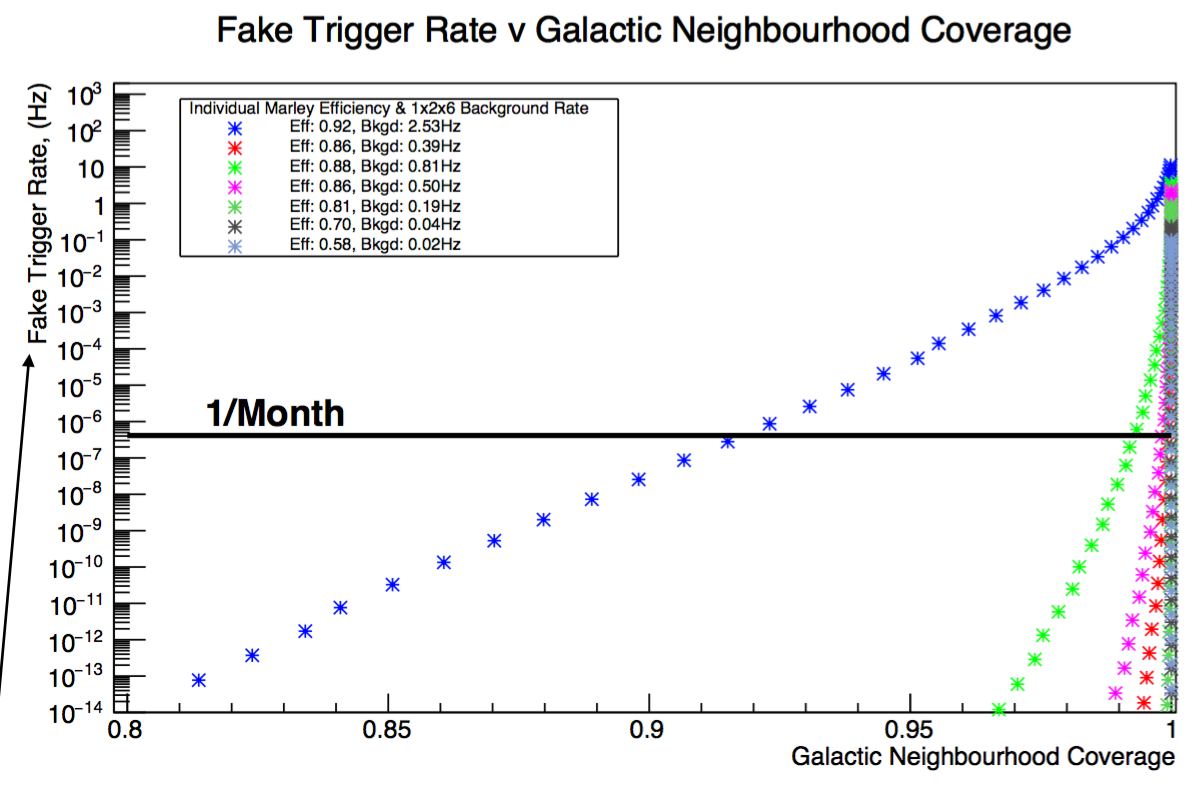
\includegraphics[width=0.9\textwidth]{images/sn_trigger.png}
% \caption{\label{fig:sntrigger} SN trigger 
% efficiency vs. fake rate for different 
% single event assumptions. Each curve assumes
% a different efficiency/fake rate pair for single neutrino events. For the full SN burst,
% very high efficiency can be obtained at fake rates less than 1/month.}
% \end{figure}

% \section{Overview of the Proposed DUNE RCE/ATCA-Based DAQ System}
% \label{sec:overview}
% %%%  Matt
% The previous section has made it clear that, in the event of a galactic SN it is desirable to save the entire, non-zero-suppressed data stream to long term storage for a period of ~100 seconds. 
% The full data stream will be about 9 Tb/s of ADC data for one single-phase 10kT module. 
% Various overheads raise this rate to between 12 and 15 Tb/s.
% The DUNE Technical Proposal assumes 12 Tb/s of TPC data, so will use that rate for the rest of this note.
% The primary data stream of the DUNE DAQ system will not be capable of writing this amount of data in "real time". 
% The back-end network and storage bandwidths would both be much larger than needed for any other type of physics, and thus would be prohibitively expensive.

% However, as discussed in Section \ref{sec:sntrigger},
% we expect to be able to trigger efficiently on galactic SN bursts with a latency of approximately one second. 
% We can imagine buffering the full datastream for 100 seconds or more in some sort of local storage upon receipt of such a trigger.
% A "look-back" buffer of several seconds length would also be needed to record the data from the time before the trigger is issued.
% Once the data for the full 100 seconds is stored, it could then be trickled out slowly to permanent storage once the burst is completed.

% In principal, one could imagine building such a buffer with DDRAM.
% However, the cost of this would be prohibitive. At current costs (10\$/GByte), this cost would be about \$15,000/second for a single 10kT TPC module. 
% For a full 100 second buffer, the total cost would be about 1.5M\$, which is unacceptably high.

% Another available technology is a Non-volatile Memory Solid State Drive (NVMe SSD). 
% This is cheaper than DDRAM by about a factor of 20 (\$0.50/GByte).  A 100-second buffer for a single module, would thus cost about 75K\$ - a very acceptable price.
% Recently, input bandwidths of NVMe devices have exceeded 2 GB/s, which allows them to match to the input bandwidth of a single front-end processor, e.g., an RCE.
% However, NVMe has a limited lifetime that is described by its "endurance".
% Endurance is measured in "Terabytes Written" (TBW), which is typically 500 to 1000 times the size of the device - meaning that the entire device can be written that many times before failure. 
% If a 100-second NVMe buffer were written to continuously, it would be expected to fail in ~100,000 seconds (about 1 day).
% Therefore, the double buffer cannot be made only of NVMe but a hybrid of pre-buffer in DRAM and post-buffer in NVMe. 